\documentclass[SoftwareDesign/SoftwareDesign_main.tex]{subfiles}

\begin{document}

\section{Design af Search}
Dette afsnit beskriver designet for henholdsvis Search View og Search ViewModel. Betegnelsen 'Search' dækker over den del af applikationen, som giver lejere mulighed for at finde og leje biler. Der er dedikeret en side i applikationen til søge funktionaliteten, og designet af denne tager udgangspunkt i en WireFrame, som kan ses i figur \ref{fig:search_wireframe}. Det fremgår, at siden er delt i to. Som bruger skal man have mulighed for at se, hvilke biler, der er tilgængelige, dvs. de biler som tidligere er blevet registreret i systemet af en udlejer, og som nu kan lejes. Dette er vist til højre i figur \ref{fig:search_wireframe}, hvor der kan scrolles gennem udvalgte biler. Hver af de adskilte enheder repræsenterer én bil og indeholder således et billede, nogle relevante informationer vedrørende bilen og en knap, som giver brugeren mulighed for at leje den. \\\\Til venstre i figur \ref{fig:search_wireframe} er en række søgekriterier, som giver brugeren mulighed for at sortere i søgeresultaterne. Dermed behøver brugeren altså ikke at gennemgå samtlige biler, men kun de relevante biler, der opfylder de indtastede kriterier. Der foretages ikke gentagne søgninger i databasen. Det vurderes, at det er en bedre løsning at foretage en enkelt søgning, og vise brugeren et udsnit eller samtlige biler i databasen, som så efterfølgende kan blive filtreret. Selv om det betegnes 'Search' er det altså filtrering af søgeresultater, som er det essentielle, og dette er en del af præsentationslogikken. Med denne fremgangsmåde mindskes interaktionen med databasen, og derved er der mindre overhead og risiko for fejl.

\begin{figure}[H]
    \centering
    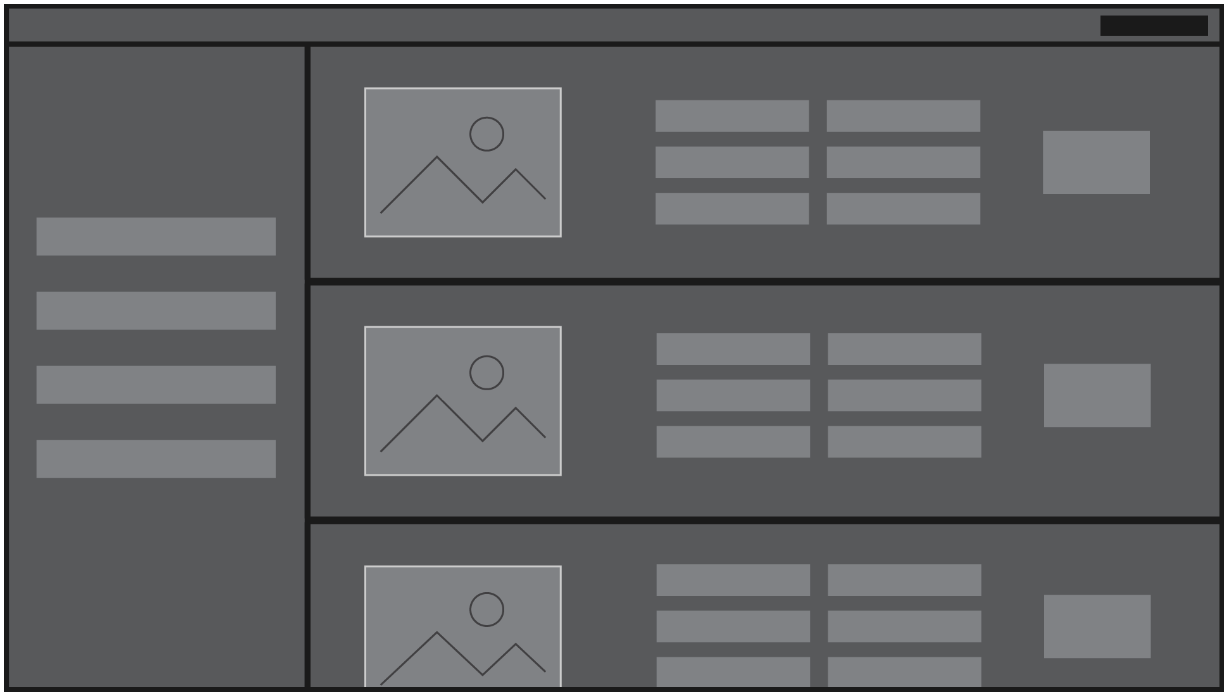
\includegraphics[width=\textwidth]{SoftwareDesign/MVVMDesigns/Graphics/SearchWireFrame.png}
    \caption{Search Page WireFrame}
    \label{fig:search_wireframe}
\end{figure}

\subsection{Design af Search View}
For at kunne vise bilerne på en hensigtsmæssig måde er der lavet en UserControl med et billede af bilen og informationer om bilmærke- og model, lokation, pris, antal sæder og udlejers navn. Disse er bundet til properties i den ViewModel, som er tilknyttet, og som repræsenterer det enkelte søgeresultat (SearchResultItem ViewModel). Informationerne trækkes ud af databasen og søgeresultaterne er initialiseret, når der navigeres til Search View. Dette indeholder desuden søgefelter for henholdsvis lokation, bilmærke, antal sæder, samt datoer for afhentning og tilbagelevering. Samtlige af disse søgekriterier er bundet til properties i den tilknyttede Search ViewModel.

\subsection{Design af Search ViewModel}
Der kan navigeres til søgevinduet ved at trykke på 'Find Car' knappen som befinder sig i Header Bar. Search ViewModel har abonneret på en EventAggregator, og derfor kan der navigeres fra Header Bar til Search uden at de har direkte kendskab til hinanden. Alternativt kan der foretages en 'hurtig-søgning' i søgefeltet i Header Bar. Dette medfører at der navigeres til Search og foretages en filtrering efter lokation på baggrund af den indtastede string. Når der trykkes på 'Rent'-knappen for en bil gøres der igen brug af Event Aggregator, og der navigeres til SendRequest View, mens bilens informationer sendes med. \\\\Search ViewModel har en ObservableCollection bestående af SearchResultItemViewModels. Det er denne, som udgør søgeresultatet, og som der bindes til i Viewet. Til selve filtreringen anvendes et CollectionView. Det giver mulighed for at manipulere den Collection, som Viewet er bundet til, mens abstraktionen mellem View og ViewModel bevares. På denne vis anvendes ObservableCollection som en form for repository, og brugeren kan frit vælge at kombinere en eller flere af søgekriterierne, som der så bliver filtreret efter ved tryk på en søge-knap. \\\\Når brugeren har indtastet en oplysning i venstre side bliver kriteriet tilføjet en liste af Predicates med den værdi, som der skal sammenlignes med. Hvis der ikke er udfyldt nogen kriterier vises alle bilerne, og ellers skal alle Predicates tjekkes og være opfyldt for en given bil før den inkluderes i Viewet. Denne fremgangsmåde har fordelen, at hvert enkelt søgekriterie kan holdes simpelt og testes separat. \\\\Search View Model realiserer interfacet IDataErrorInfo med det formål at håndtere fejl. Data valideres bl.a. når der indtastes antal sæder eller vælges datoer i venstre side af Search View. Hvis ikke der er valgt en gyldig værdi, får tekstboksen en rød kant, og der bliver udstedt en passende fejlmeddelse i tooltip. Det vil desuden heller ikke være muligt at foretage en søgning, hvis der er kriterier med ugyldig data.

\end{document}